\documentclass[12pt,a4paper]{article}
\usepackage{graphicx}
\usepackage[table]{xcolor}
\usepackage{circuitikz}
\usepackage{amsmath}
\usepackage[spanish]{babel}
\usepackage[utf8]{inputenc}
\usepackage[T1]{fontenc}
\usepackage{subcaption}
\usepackage[hidelinks]{hyperref}
\usepackage{siunitx}
\usepackage{booktabs}
\usepackage{caption}
\usepackage[version=4]{mhchem}
\usepackage{float} 
\usepackage{graphicx}
\usepackage{geometry}
\usepackage{setspace}
\usepackage{needspace}
\usepackage{algorithm}
\usepackage{algpseudocode}
\definecolor{algorithmblue}{HTML}{175676}
\definecolor{algorithmgray}{HTML}{68737D}
\floatstyle{ruled}
\restylefloat{algorithm}
\captionsetup[algorithm]{labelfont={bf,color=algorithmblue},textfont=it,skip=6pt}
\algrenewcommand{\algorithmicprocedure}{\textbf{\color{algorithmblue}Procedimiento}}
\algrenewcommand{\algorithmicdo}{\textbf{hacer}}
\algrenewcommand{\alglinenumber}[1]{\tiny\color{algorithmgray}\makebox[1.8em][r]{#1}}
\graphicspath{{Imagenes/}}
% Márgenes normales del documento
\geometry{
left=2.5cm, 
right=2.5cm,
top=2.5cm,
bottom=2.5cm
}

\setlength{\parskip}{0.2\baselineskip}

\begin{document}

\begin{center}

% para recortar el logo

\includegraphics[
width=\textwidth,
trim=0cm 1.9cm 0cm 1.9cm,
clip
]{Logo.png}

\vspace{-0.35cm}

\rule{\textwidth}{0.4pt}

\vspace{-0.1cm}

{\small \textbf{Practica No.08}}

\vspace{0.1cm}

{\LARGE \textbf{Configuración de diodos con entradas en DC}}

\vspace{0.1cm}

{\itshape Enriquez Yussed, Enriquez Andres, Tarapuez Juan y Tarapues German}

\vspace{-0.2cm}

\href{mailto:acenriquez24b@udenar.edu.co}{acenriquez24b@udenar.edu.co} /
\href{mailto:ayes0317@gmail.com}{ayes0317@gmail.com}\\
\href{mailto:juandatara89ljfj@gmail.com}{juandatara89ljfj@gmail.com} /
\href{mailto:edisongtarapues04@gmail.com}{edisongtarapues04@gmail.com}

\vspace{0.1cm}

\textbf{Laboratorio de Fundamentos de Electronica, Física, Universidad de Nariño, 
31/octubre/26}

\vspace{0.1cm}

\rule{\textwidth}{0.4pt}

\end{center}

\vspace{0.4cm}

\begin{abstract}
Comprobar experimentalmente la validez de la segunda aproximación del diodo 
semiconductor, que modela el diodo como un diodo ideal en serie con una batería de 
0,7 V para el silicio y 0,3 V para el germanio, aplicada a diferentes configuraciones 
de diodos alimentadas con corriente continua. Se analizaron cuatro circuitos: un diodo 
de silicio en serie con una resistencia, con polarización directa e inversa; un arreglo 
en serie de diodos de silicio y germanio; un arreglo de diodos de silicio y germanio en 
paralelo; y un circuito con dos diodos de silicio y dos resistencias. Para cada circuito 
se resolvió teóricamente el voltaje en los diodos y en las resistencias, y las corrientes, 
usando las leyes de Kirchhoff. Luego se midieron estas mismas magnitudes con un multímetro 
digital, se compararon con los valores teóricos y se aplicó la Teoría de Errores a los resultados 
experimentales para evaluar el alcance y las limitaciones del modelo propuesto.

\end{abstract}

\input{Capitulos/introduccion.tex}

\section{Marco Teórico}

\subsection{Conductores eléctricos}

Son materiales que ofrecen poca resistencia al movimiento de la carga eléctrica. Sus \textbf{átomos} se caracterizan por tener pocos electrones en su \textbf{capa de valencia}, por lo que no se necesita mucha energía para que estos salten de un átomo a otro.

También se considera conductor eléctrico a cualquier cuerpo formado por \textbf{materia eléctricamente conductora}. Se distinguen dos tipos principales de conductores:

\begin{figure}[h]
    \centering
    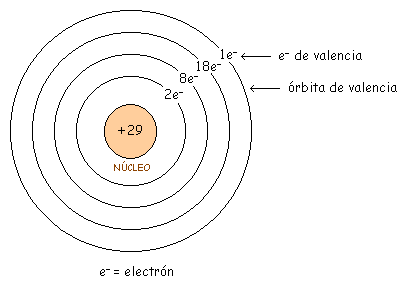
\includegraphics[width=0.5\textwidth]{images.png}
    \caption{Representación del electrón de valencia en un átomo conductor.}
    \label{fig:atomo_valencia}
\end{figure}

\begin{itemize}
    \item \textbf{Conductor Homogéneo:} Son aquellos materiales o cables eléctricos cuya conductividad y composición son uniformes en todos sus puntos.
    \item \textbf{Conductor Combinado:} (O conductor bimetálico/compuesto) Son aquellos fabricados mediante la combinación de dos materiales diferentes (por ejemplo, aluminio y acero, o cobre y acero) para aprovechar las propiedades mecánicas de uno y las eléctricas del otro.
\end{itemize}

\begin{table}[h]
    \centering
    \caption{Resistividad de los conductores más comunes a $20\,^{\circ}\text{C}$}
    \label{tab:conductores}
    \begin{tabular}{|l|c|c|}
        \hline
        \textbf{Material} & \textbf{Símbolo} & \textbf{Resistividad ($\times 10^{-8} \ \Omega \cdot \text{m}$)} \\ \hline
        Plata    & Ag & 1.64  \\ \hline
        Cobre    & Cu & 1.72  \\ \hline
        Oro      & Au & 2.45  \\ \hline
        Aluminio & Al & 2.82  \\ \hline
        Hierro   & Fe & 8.90  \\ \hline
        Estaño   & Sn & 11.50 \\ \hline
        Grafito  & C  & 60.00 \\ \hline
    \end{tabular}
\end{table}

\subsection{Aislantes eléctricos}

Son materiales que presentan una gran resistencia al movimiento de la carga eléctrica, impidiendo el flujo libre de los electrones. Sus \textbf{átomos} se caracterizan por tener sus \textbf{capas de valencia} completas o casi llenas, lo que genera una fuerza de atracción nuclear muy intensa sobre los electrones, requiriendo niveles extremadamente altos de energía para moverlos.

También se conocen como dieléctricos y son fundamentales para la seguridad y confinamiento de la corriente. Se distinguen dos categorías según su origen y aplicación:


\begin{figure}[h]
    \centering
    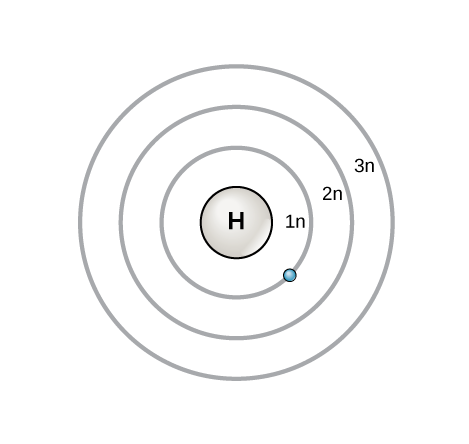
\includegraphics[width=0.5\textwidth]{aislante_atomo.png}
    \caption{Estructura atómica de un aislante con su capa de valencia completa, impidiendo el flujo de electrones.}
    \label{fig:atomo_aislante}
\end{figure}


\begin{itemize}
    \item \textbf{Aislantes Sólidos:} Son materiales compactos de alta rigidez dieléctrica que se utilizan para recubrir o soportar físicamente las estructuras conductoras (por ejemplo, el vidrio, la cerámica o polímeros como el PVC).
    \item \textbf{Aislantes Líquidos o Gaseosos:} Son fluidos utilizados en aplicaciones industriales de alta potencia, como transformadores, para aislar y disipar calor de forma simultánea (por ejemplo, el aceite mineral o el gas hexafluoruro de azufre).
\end{itemize}

\begin{table}[h]
    \centering
    \caption{Resistividad de los aislantes más comunes a $20\,^{\circ}\text{C}$}
    \label{tab:aislantes}
    \begin{tabular}{|l|c|c|}
        \hline
        \textbf{Material} & \textbf{Fórmula / Tipo} & \textbf{Resistividad ($\Omega \cdot \text{m}$)} \\ \hline
        Agua destilada & H$_2$O & $2 \times 10^{5}$ \\ \hline
        Vidrio         & SiO$_2$ (base) & $10^{10} - 10^{14}$ \\ \hline
        Goma dura      & Polímero & $10^{13}$ \\ \hline
        Azufre         & S & $10^{15}$ \\ \hline
        Teflón         & (C$_2$F$_4$)$_n$ & $10^{22} - 10^{24}$ \\ \hline
    \end{tabular}
\end{table}

\subsection{Semiconductores eléctricos}

Son materiales que poseen propiedades eléctricas intermedias entre los conductores y los aislantes. Sus \textbf{átomos} se caracterizan por tener exactamente cuatro electrones en su \textbf{capa de valencia}. Bajo condiciones normales actúan como aislantes, pero al recibir energía externa (calor, luz o un voltaje aplicado) o mediante el proceso de dopado, sus electrones pueden saltar con relativa facilidad a la banda de conducción.

El Silicio es el elemento semiconductor más utilizado en la industria electrónica para la fabricación de diodos, transistores y circuitos integrados. Dependiendo de su pureza y tratamiento, se clasifican en dos tipos principales:

\begin{itemize}
    \item \textbf{Semiconductores Intrínsecos:} Son aquellos materiales que se encuentran en un estado puro, sin ningún tipo de impurezas en su estructura cristalina (como el silicio o germanio puros a temperatura ambiente).
    \item \textbf{Semiconductores Extrínsecos:} Son aquellos que han sido modificados mediante la introducción deliberada de átomos de otros elementos (proceso de dopado) para alterar drásticamente su conductividad, dividiéndose en tipo P (aceptadores de electrones) y tipo N (donadores de electrones).
\end{itemize}

\begin{figure}[h]
    \centering
    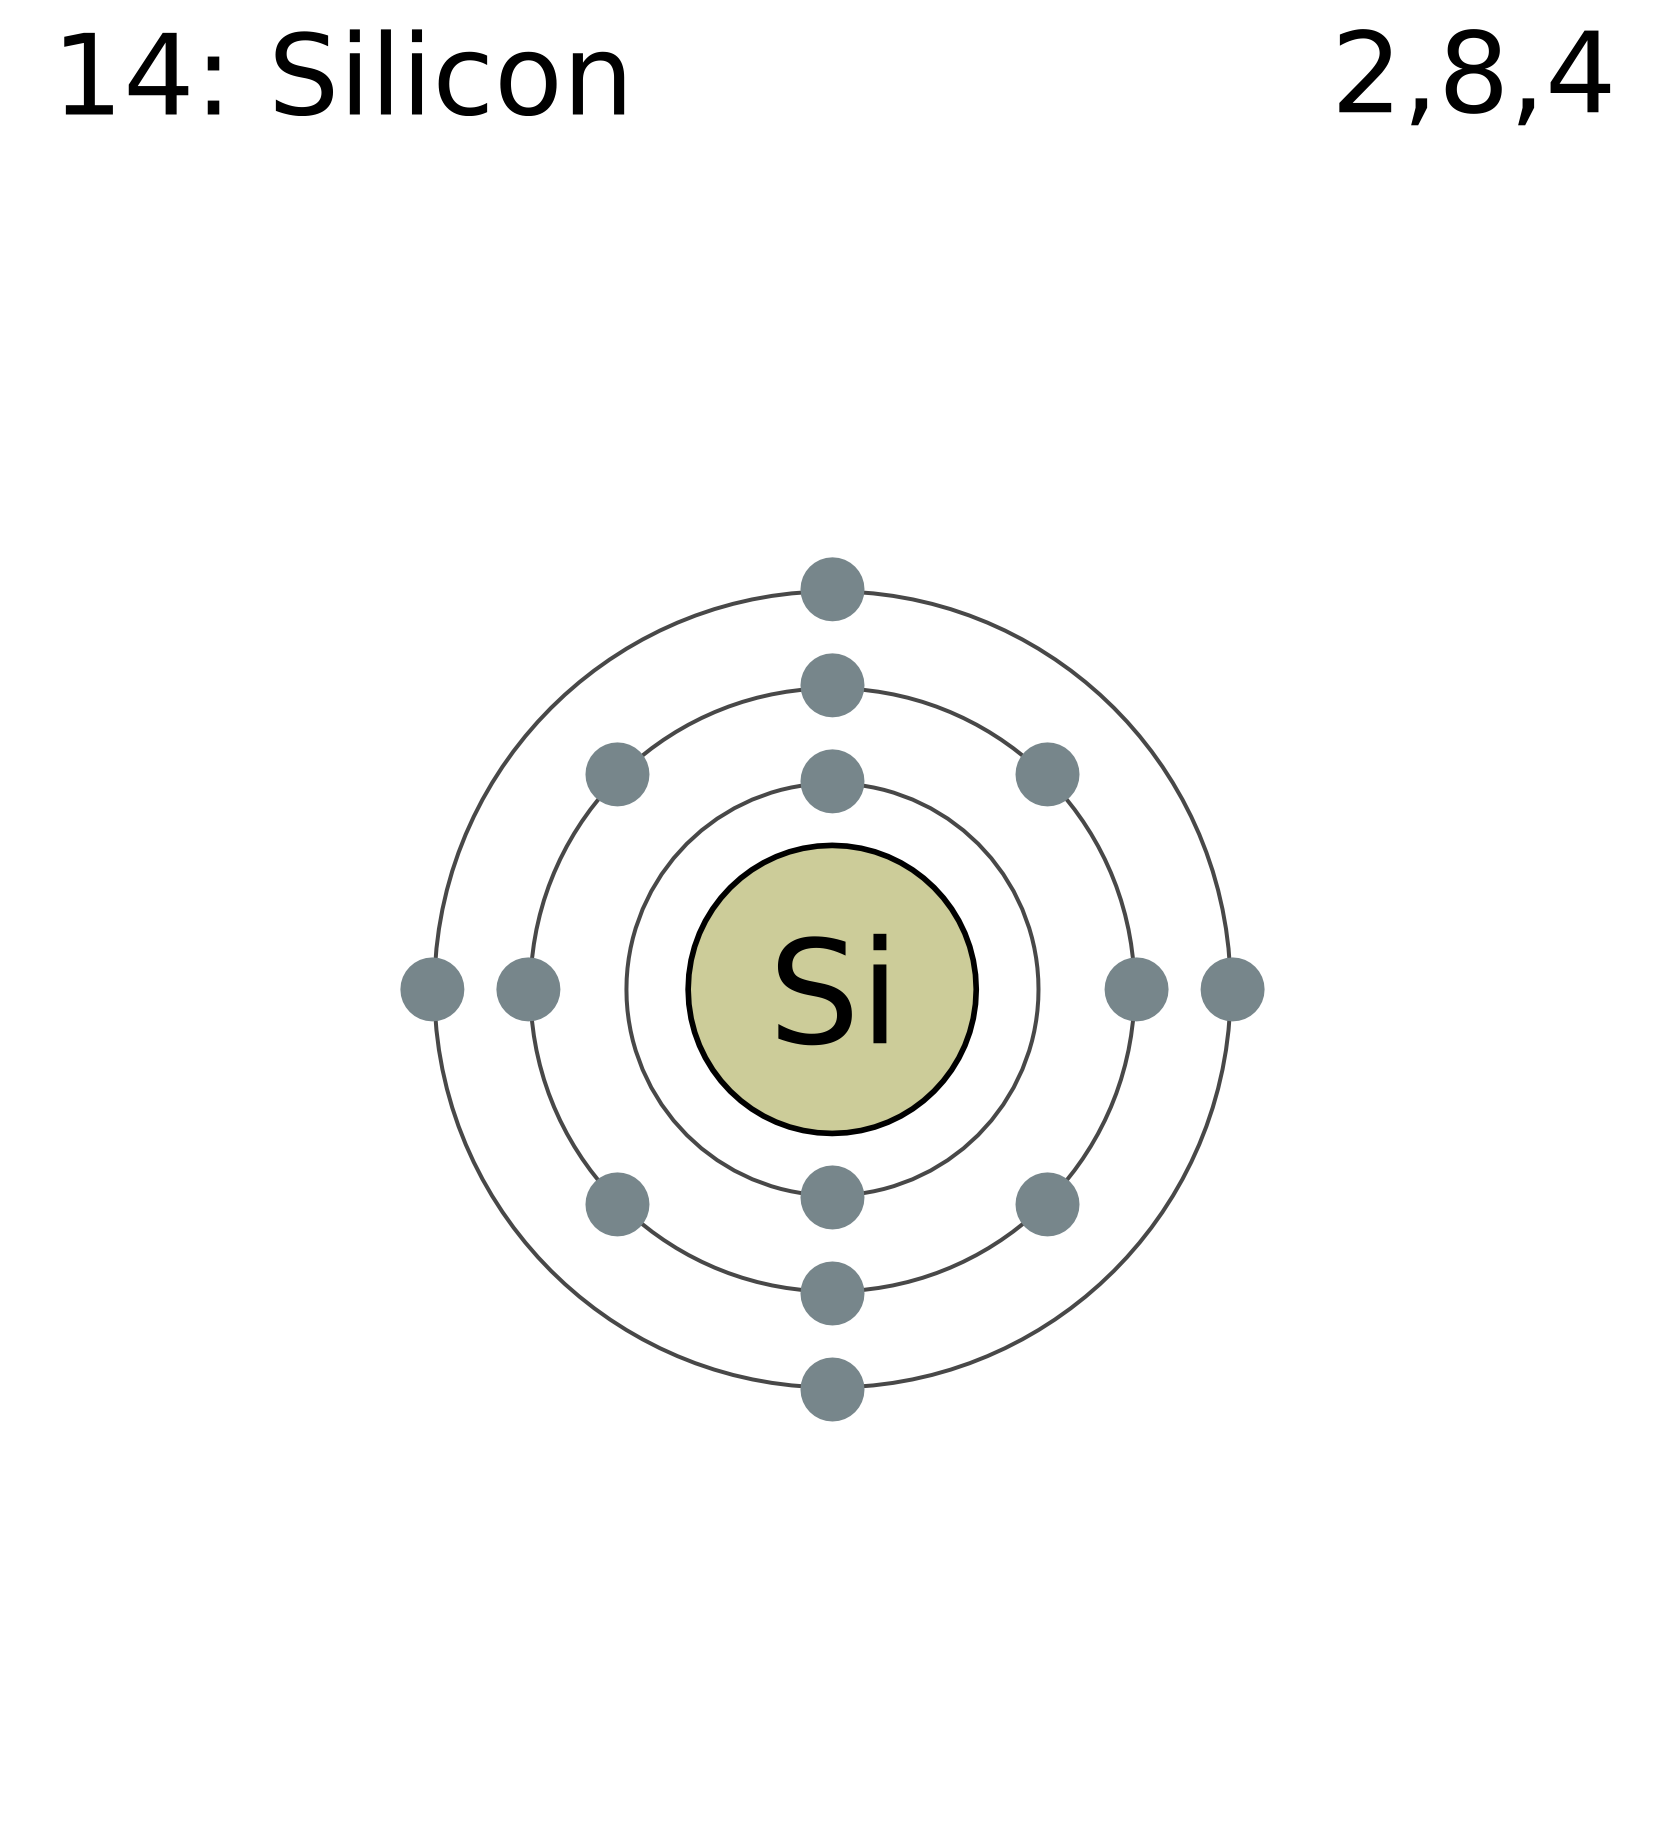
\includegraphics[width=0.45\textwidth]{silicio_atomo.png}
    \caption{Representación del modelo atómico del Silicio (Si) destacando sus cuatro electrones de valencia.}
    \label{fig:atomo_silicio}
\end{figure}

\begin{table}[h]
    \centering
    \caption{Resistividad de los semiconductores más comunes a $20\,^{\circ}\text{C}$}
    \label{tab:semiconductores}
    \begin{tabular}{|l|c|c|}
        \hline
        \textbf{Material} & \textbf{Símbolo} & \textbf{Resistividad ($\Omega \cdot \text{m}$)} \\ \hline
        Germanio & Ge & 0.46 \\ \hline
        Silicio  & Si & $2.3 \times 10^{3}$ \\ \hline
    \end{tabular}
\end{table}


\subsection{Semiconductores Intrínsecos y Equilibrio Térmico}
Un semiconductor intrínseco define a un material semiconductor en su estado de máxima pureza química, libre de defectos estructurales o impurezas intencionadas en su red cristalina. A la temperatura del cero absoluto ($0\text{ K}$), el material se comporta como un aislante perfecto debido a que todos los electrones de valencia se encuentran confinados en los enlaces covalentes que configuran la estructura del cristal.

Al incrementarse la temperatura ambiente ($T > 0\text{ K}$), la agitación térmica aporta la energía mínima necesaria para romper una fracción de estos enlaces covalentes. Este fenómeno físico provoca que un electrón adquiera la energía suficiente para superar la banda prohibida o \textit{bandgap} ($E_g$) y transite hacia la banda de conducción, transformándose en un electrón libre. Simultáneamente, la ausencia del electrón en el enlace covalente original genera una vacante con carga positiva neta en la banda de valencia, denominada mecánicamente como \textit{hueco}.

Este mecanismo se conoce como generación térmica de pares electrón-hueco. Dado que cada electrón libre genera de manera unívoca un hueco, en condiciones de equilibrio térmico se establece que la densidad de electrones libres ($n$) es estrictamente igual a la densidad de huecos ($p$), e igual a la concentración intrínseca del portador ($n_i$):

\begin{equation}
n = p = n_i
\end{equation}

La concentración intrínseca es una propiedad intrínseca del material dependiente de la temperatura y de la magnitud de su banda prohibida, gobernada por la siguiente relación matemática:

\begin{equation}
n_i^2 = N_c N_v \exp\left(-\frac{E_g}{k_B T}\right)
\end{equation}

Donde $N_c$ y $N_v$ representan las densidades efectivas de estados en las bandas de conducción y valencia respectivamente, $k_B$ es la constante de Boltzmann y $T$ es la temperatura absoluta en Kelvin.

\subsection{Semiconductores Extrínsecos: El Proceso de Dopaje}
Debido a que la conductividad eléctrica de un semiconductor intrínseco es extremadamente baja a temperatura ambiente para aplicaciones prácticas, se recurre al proceso de dopaje. Este consiste en la introducción controlada de átomos de impurezas en la red cristalina para alterar deliberadamente las concentraciones de portadores de carga, dando origen a los semiconductores extrínsecos.

\subsubsection{Semiconductores Tipo N (Negativo)}
Se obtienen mediante la introducción de impurezas pentavalentes, es decir, átomos pertenecientes al Grupo V de la tabla periódica (tales como el Fósforo, $\text{P}$, o el Arsénico, $\text{As}$) en una matriz de silicio tetravalente. Al sustituir un átomo de silicio, la impureza emplea cuatro de sus electrones de valencia para consolidar los enlaces covalentes con los átomos adyacentes. El quinto electrón queda libre de enlace y requiere una energía de ionización muy baja para situarse en la banda de conducción.

A estas impurezas se les denomina \textit{átomos donadores}. En consecuencia, en un semiconductor Tipo N, los \textbf{electrones libres} constituyen los portadores mayoritarios ($n \gg p$), mientras que los huecos pasan a ser los portadores minoritarios.

\subsubsection{Semiconductores Tipo P (Positivo)}
Se producen mediante la adición de impurezas trivalentes del Grupo III de la tabla periódica (como el Boro, $\text{B}$, o el Galio, $\text{Ga}$). Al insertarse en la estructura del silicio, el átomo dopante dispone únicamente de tres electrones, dejando uno de los cuatro enlaces covalentes vecino incompleto. Esta deficiencia electrónica genera un nivel de energía vacío estable que actúa como un \textit{hueco} capaz de aceptar un electrón de la banda de valencia.

Estas impurezas reciben el nombre de \textit{átomos aceptores}. Por consiguiente, en un semiconductor Tipo P, los \textbf{huecos} representan los portadores mayoritarios ($p \gg n$), mientras que los electrones libres actúan como portadores minoritarios.

\begin{figure}[htbp]
    \centering
    \begin{subfigure}[b]{0.45\textwidth}
        \centering
        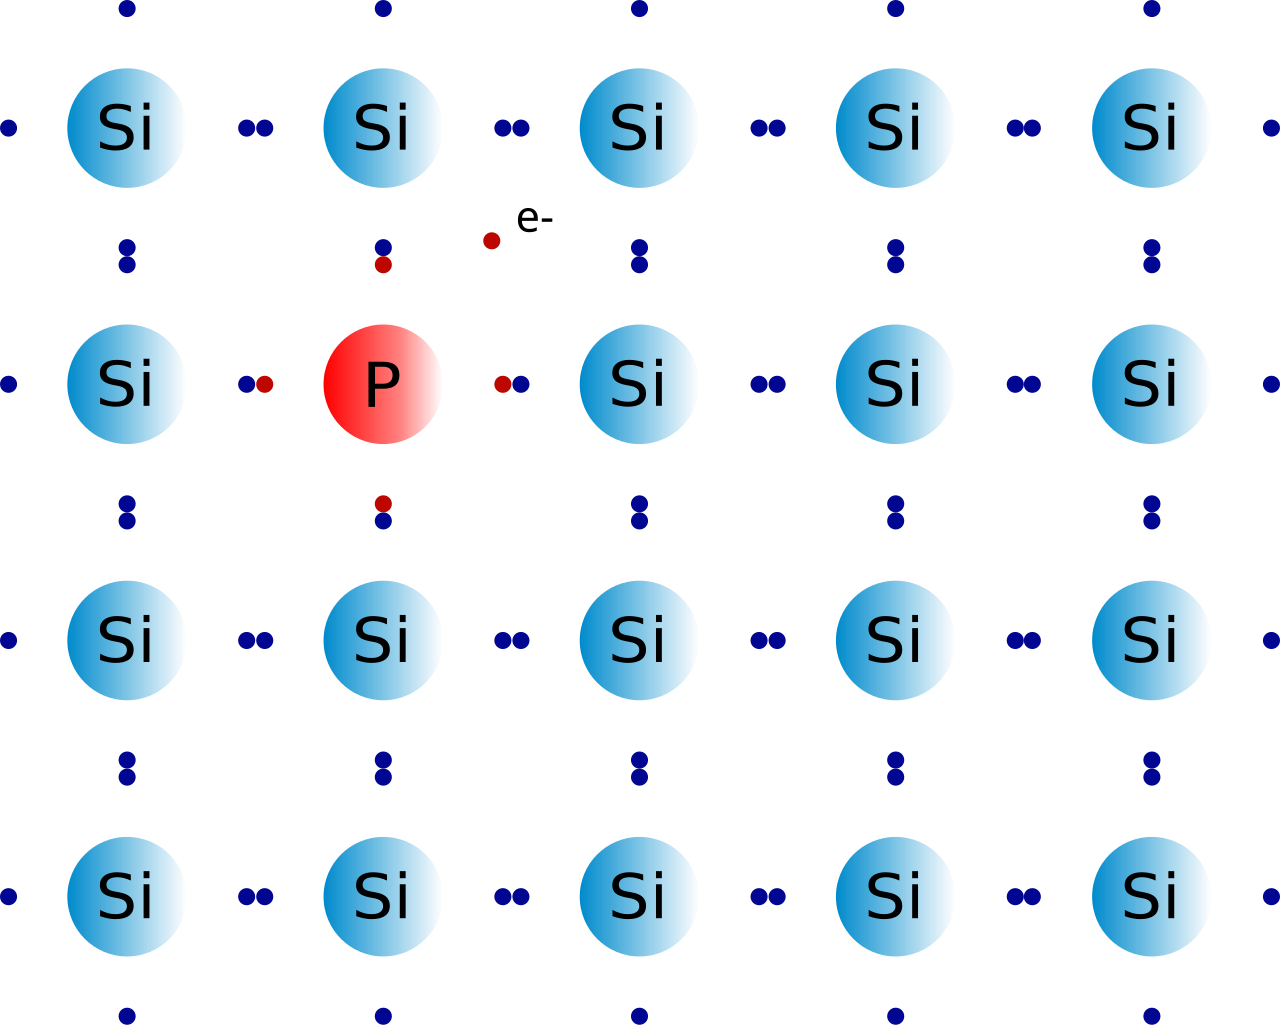
\includegraphics[width=\textwidth]{dopaje_n.png}
        \caption{Dopaje Tipo N: Átomo pentavalente (Fósforo) aportando un electrón libre a la red.}
        \label{fig:dopaje_n}
    \end{subfigure}
    \hfill
    \begin{subfigure}[b]{0.45\textwidth}
        \centering
        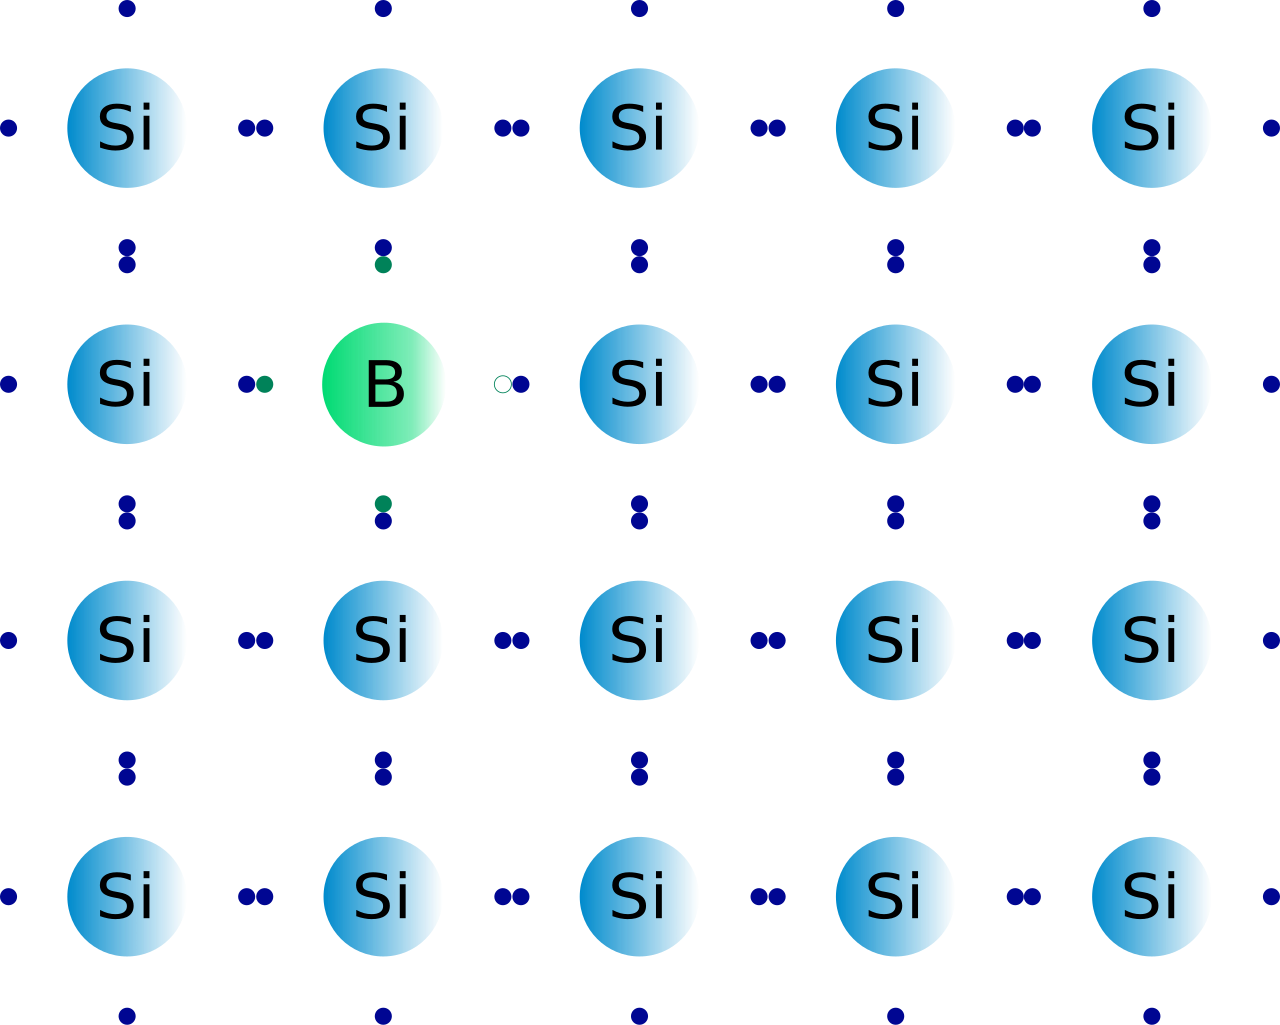
\includegraphics[width=\textwidth]{dopaje_p.png}
        \caption{Dopaje Tipo P: Átomo trivalente (Boro) generando un hueco en la red covalente.}
        \label{fig:dopaje_p}
    \end{subfigure}
    \caption{Representación bidimensional de la estructura cristalina del silicio modificado mediante dopaje extrínseco.}
    \label{fig:dopajes_extrinsecos}
\end{figure}

\subsection{La Unión P-N y la Región de Agotamiento}
Cuando un cristal semiconductor Tipo P se une de manera atómica con un cristal Tipo N, se genera una interfaz crítica conocida como unión P-N. Debido al abrupto gradiente de concentración en la frontera, los electrones libres de la región N difunden hacia la región P, mientras que los huecos de la región P difunden hacia la región N. Este desplazamiento macroscópico de cargas provoca la combinación inmediata de electrones y huecos en las proximidades de la interfaz, proceso denominado \textit{recombinación}.

Como consecuencia directa de la recombinación en la frontera:
\begin{itemize}
    \item Los átomos donadores en el lado N pierden su electrón libre y se transforman en \textbf{iones positivos fijos}.
    \item Los átomos aceptores en el lado P capturan un electrón y se transforman en \textbf{iones negativos fijos}.
\end{itemize}

Esta transferencia espacial de carga despoja a la interfaz de sus portadores móviles, instaurando una zona desprovista de conducción denominada \textbf{región de agotamiento} (o región de carga espacial). Los iones fijos e inmóviles remanentes en esta zona inducen un campo eléctrico interno direccionado desde el lado N hacia el lado P. Este campo eléctrico genera una barrera de potencial invisible (aproximadamente $0.7\text{ V}$ para el silicio) que se opone de forma idónea a una mayor difusión de portadores mayoritarios, estableciendo un estado de equilibrio dinámico.

\subsection{Regímenes de Polarización de la Unión P-N}
El comportamiento eléctrico de la unión P-N se modifica drásticamente mediante la aplicación de una diferencia de potencial externa ($V_a$):

\begin{figure}[htbp]
    \centering
    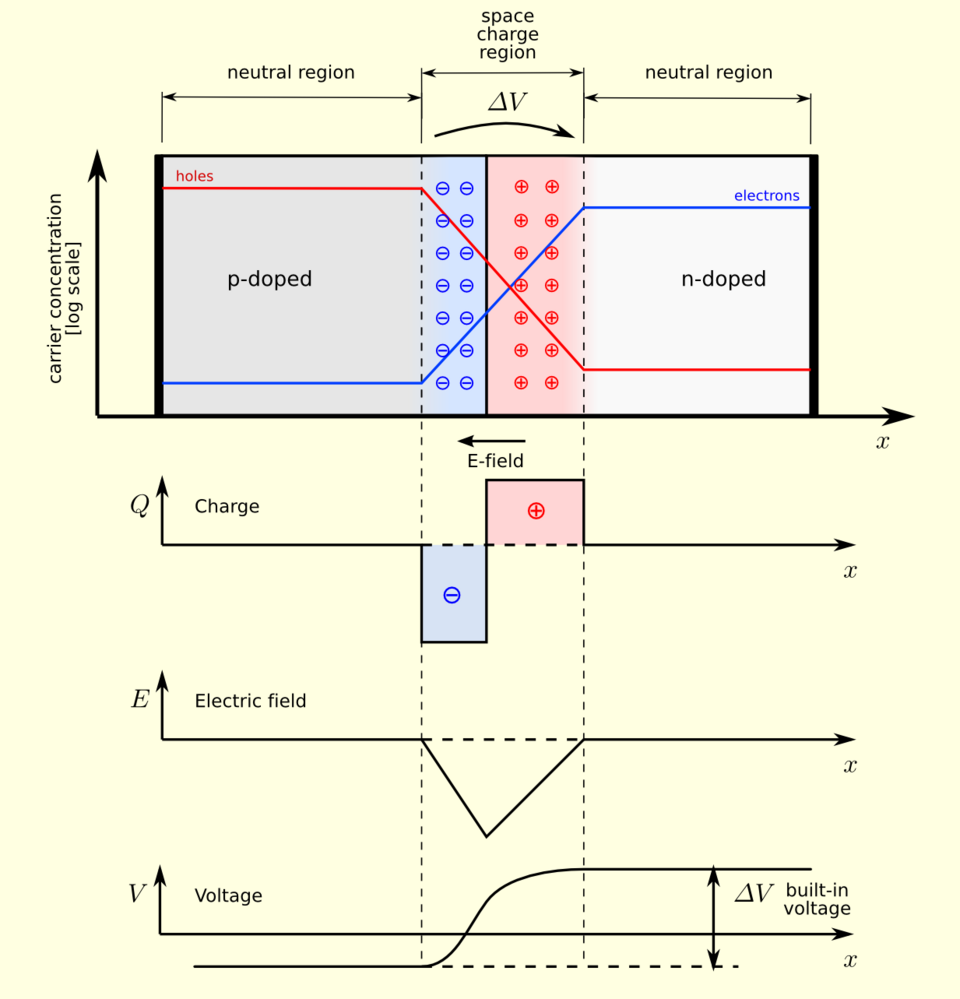
\includegraphics[width=0.75\textwidth]{region_agotamiento.png}
    \caption{Diagrama esquemático de la unión P-N en equilibrio térmico, destacando la formación de la región de agotamiento poblada por iones fijos y el campo eléctrico interno resultante.}
    \label{fig:region_agotamiento}
\end{figure}


\subsubsection{Polarización Directa}
Ocurre al conectar el terminal positivo de una fuente externa a la región P y el terminal negativo a la región N ($V_a > 0$). El campo eléctrico externo se opone directamente al campo eléctrico interno de la unión. Esto reduce el ancho de la región de agotamiento y disminuye notablemente la barrera de potencial. Cuando el voltaje externo supera el potencial de barrera, los portadores mayoritarios adquieren la energía cinética suficiente para cruzar la unión en masa, permitiendo un flujo de corriente eléctrica de carácter exponencial.

\subsubsection{Polarización Inversa}
Se presenta al conectar el terminal positivo de la fuente a la región N y el terminal negativo a la región P ($V_a < 0$). En este régimen, el campo eléctrico externo se alinea vectorialmente con el campo interno, atrayendo a los portadores mayoritarios hacia los extremos del dispositivo. Como resultado, la región de agotamiento se ensancha significativamente y la barrera de potencial aumenta de forma drástica, bloqueando el paso de los portadores mayoritarios.

La corriente total en este estado no es estrictamente cero; se manifiesta una corriente de magnitud minúscula (del orden de los nanoamperios) denominada \textit{corriente de saturación inversa} o corriente de fuga ($I_0$). Esta corriente se debe exclusivamente al arrastre de los portadores minoritarios a través de la unión, generados térmicamente en el material.

\subsection{El Diodo Zener y el Fenómeno de Ruptura Inversa}
Si el voltaje en polarización inversa se incrementa más allá de un límite crítico específico, conocido como voltaje de ruptura ($V_Z$), el campo eléctrico en la región de agotamiento alcanza una intensidad crítica capaz de arrancar electrones directamente de los enlaces covalentes (efecto Zener) o de acelerar electrones minoritarios con suficiente energía para ionizar otros átomos por impacto en cadena (efecto avalancha).

A diferencia de un diodo convencional de la unión P-N, el cual sufre una destrucción térmica irreversible bajo estas condiciones, el \textbf{diodo Zener} se fabrica con perfiles de dopaje altamente concentrados para operar de forma segura y continua dentro de esta región de ruptura inversa. Al alcanzar el potencial $V_Z$, la corriente inversa se incrementa de forma abrupta mientras que la caída de tensión en los terminales del dispositivo permanece prácticamente constante. Esta propiedad fundamental convierte al diodo Zener en el componente idóneo para aplicaciones de regulación de tensión y protección contra sobrevoltajes en sistemas electrónicos.


\subsection{La Corriente de Saturación Inversa ($I_0$)}
Como se estableció previamente, cuando una unión P-N se somete a un régimen de polarización inversa, el flujo de portadores mayoritarios queda bloqueado por el incremento de la barrera de potencial. No obstante, se manifiesta una corriente eléctrica residual de magnitud infinitesimal denominada \textit{corriente de saturación inversa} o corriente de fuga ($I_0$).

Esta corriente es de naturaleza puramente térmica y es conducida exclusivamente por los portadores minoritarios (electrones libres en la región P y huecos en la región N) que son arrastrados a través de la región de agotamiento por el campo eléctrico aplicado. La relación matemática que gobierna la corriente total ($I$) en un diodo a lo largo de todos sus regímenes operativos viene descrita por la ecuación ideal de diodo de Shockley:

\begin{equation}
I = I_0 \left( \exp\left(\frac{q V_a}{n k_B T}\right) - 1 \right)
\end{equation}

Donde $V_a$ representa el voltaje neto aplicado a los terminales del componente, $q$ es la carga elemental del electrón ($1.602 \times 10^{-19}\text{ C}$), $k_B$ representa la constante de Boltzmann, $T$ es la temperatura absoluta en Kelvin y $n$ define el factor de idealidad del semiconductor (cuyo valor oscila típicamente entre $1$ y $2$ dependiendo del material y del nivel de dopaje). Cuando el diodo está polarizado en inversa ($V_a < 0$), el término exponencial decrece exponencialmente hacia cero, haciendo que la corriente total se estabilice en el valor constante e inverso de $-I_0$.

\subsection{Modelos de Aproximación Eléctrica del Diodo}
Con la finalidad de simplificar el análisis y modelado matemático de los diodos de unión P-N en el diseño de circuitos prácticos, la curva característica exponencial real se simplifica mediante aproximaciones lineales por tramos.

\subsubsection{Primera Aproximación: Modelo del Diodo Ideal}
La primera aproximación asume que el diodo se comporta de forma ideal, comportándose como un interruptor perfecto sin pérdidas de energía ni caídas de tensión internas:
\begin{itemize}
    \item \textbf{Polarización Directa ($V_a \geq 0$):} El componente actúa como un cortocircuito (interruptor cerrado), presentando una resistencia interna nula y una caída de voltaje de exactamente $0\text{ V}$.
    \item \textbf{Polarización Inversa ($V_a < 0$):} El componente actúa como un circuito abierto (interruptor abierto), exhibiendo una resistencia infinita y permitiendo una corriente de fuga estrictamente igual a $0\text{ A}$.
\end{itemize}

La \ref{fig:primera_aproximacion} ilustra los circuitos equivalentes correspondientes a este modelo ideal elemental.

\begin{figure}[htbp]
    \centering
    \begin{subfigure}[b]{0.45\textwidth}
        \centering
        \begin{circuitikz}[scale=0.8]
            \draw (0,0) to[battery2, l=$E$] (0,2)
                  (0,2) to[short] (1,2)
                  (1,2) to[short, -*] (1.5,2)
                  (2,2) to[short, *-] (2.5,2)
                  (2.5,2) to[R, l=$R$] (2.5,0)
                  (2.5,0) -- (0,0);
            \node[above] at (1.75,2) {Ideal};
            \draw[red, thick] (1.5,2) -- (2,2); % Interruptor cerrado
        \end{circuitikz}
        \caption{Equivalente en Polarización Directa.}
    \end{subfigure}
    \hfill
    \begin{subfigure}[b]{0.45\textwidth}
        \centering
        \begin{circuitikz}[scale=0.8]
            \draw (0,0) to[battery2, l=$E$] (0,2)
                  (0,2) to[short] (1,2)
                  (1,2) to[short, -*] (1.5,2)
                  (2.2,2.3) to[short, *-] (2.5,2) % Interruptor abierto
                  (2.5,2) to[R, l=$R$] (2.5,0)
                  (2.5,0) -- (0,0);
            \node[above] at (1.75,2) {Ideal};
        \end{circuitikz}
        \caption{Equivalente en Polarización Inversa.}
    \end{subfigure}
    \caption{Modelos de circuito equivalentes para la primera aproximación (diodo ideal).}
    \label{fig:primera_aproximacion}
\end{figure}

\subsubsection{Segunda Aproximación: Modelo de Caída de Tensión Constante}
La segunda aproximación añade realismo al análisis al incorporar la existencia de la barrera de potencial intrínseca engendrada en la región de agotamiento (el potencial de contacto incorporado). Para silicio cristalino, este umbral se estipula de forma estándar en $0.7\text{ V}$.
\begin{itemize}
    \item \textbf{Polarización Directa ($V_a \geq 0.7\text{ V}$):} El diodo entra en régimen de conducción activa una vez que el potencial externo supera el umbral. Se modela matemáticamente como una \textbf{fuente de voltaje continua fija de $0.7\text{ V}$} opuesta a la fuente principal del lazo, en serie con un interruptor ideal cerrado.
    \item \textbf{Polarización Inversa ($V_a < 0.7\text{ V}$):} Si el voltaje de la malla no logra vencer la barrera de energía, el diodo permanece apagado y se modela idénticamente como un circuito abierto (interruptor abierto).
\end{itemize}

Los circuitos eléctricos equivalentes de este modelo se exponen en la \ref{fig:segunda_aproximacion}.

\begin{figure}[htbp]
    \centering
    \begin{subfigure}[b]{0.45\textwidth}
        \centering
        \begin{circuitikz}[scale=0.8]
            \draw (0,0) to[battery2, l=$E$] (0,2)
                  (0,2) to[battery2, l=$0.7\text{ V}$] (1.5,2) % Fuente de 0.7V
                  (1.5,2) to[short] (2.5,2)
                  (2.5,2) to[R, l=$R$] (2.5,0)
                  (2.5,0) -- (0,0);
        \end{circuitikz}
        \caption{Equivalente en Polarización Directa.}
    \end{subfigure}
    \hfill
    \begin{subfigure}[b]{0.45\textwidth}
        \centering
        \begin{circuitikz}[scale=0.8]
            \draw (0,0) to[battery2, l=$E$] (0,2)
                  (0,2) to[short] (1,2)
                  (1,2) to[short, -*] (1.5,2)
                  (2.2,2.3) to[short, *-] (2.5,2) % Interruptor abierto
                  (2.5,2) to[R, l=$R$] (2.5,0)
                  (2.5,0) -- (0,0);
        \end{circuitikz}
        \caption{Equivalente en Polarización Inversa.}
    \end{subfigure}
    \caption{Modelos de circuito equivalentes para la segunda aproximación (barrera de potencial).}
    \label{fig:segunda_aproximacion}
\end{figure}





























\vspace{0.5cm}

\input{Capitulos/metodologia.tex}

\vspace{0.5cm}

\input{Capitulos/resultados.tex}

\vspace{0.5cm}

\section{Preguntas}

\begin{enumerate}
    \item El material semiconductor más común es: \underline{\textbf{el Silicio (Si)}}.
    \\ \textit{\small\textbf{Razón:} El silicio es abundante en la corteza terrestre, posee excelentes propiedades mecánicas y térmicas, y presenta una banda prohibida ideal para la estabilidad operativa en un amplio rango de temperaturas.}

    \item El germanio y el silicio, en forma pura, son: \underline{\textbf{semiconductores intrínsecos}}.
    \\ \textit{\small\textbf{Razón:} Por definición, un semiconductor intrínseco representa al material en su estado de máxima pureza química, donde sus portadores eléctricos se deben únicamente a la generación térmica de pares electrón-hueco.}

    \item En el silicio dopado con impurezas como el arsénico hay una cantidad mayor de portadores de carga \underline{\textbf{electrones}} y el material es tipo \underline{\textbf{N}}.
    \\ \textit{\small\textbf{Razón:} El arsénico es una impureza pentavalente (5 electrones de valencia). Cuatro electrones forman enlaces covalentes con el silicio y el quinto queda libre en la banda de conducción, inundando el cristal de cargas negativas.}

    \item El diodo de unión puede compararse con una resistencia ya que permite el flujo de la corriente en ambas direcciones. \underline{\textbf{( F )}}
    \\ \textit{\small\textbf{Razón:} Falso. A diferencia de una resistencia lineal bilateral, el diodo es un dispositivo unidireccional no lineal que conduce corriente exponencialmente en polarización directa y bloquea el flujo en polarización inversa.}

    \item Para polarizar directamente un diodo de unión, conecte la punta \underline{\textbf{positiva}} de una batería con la terminal tipo P y la punta \underline{\textbf{negativa}} con la terminal tipo N.
    \\ \textit{\small\textbf{Razón:} Esto alinea los campos eléctricos externos opuestos al potencial interno de la unión, contrayendo la región de agotamiento para permitir la inyección masiva de portadores.}

    \item El voltaje de polarización directa de un diodo de silicio debe ser igual o mayor que \underline{\textbf{0.7}} V para que el diodo pueda conducir de manera apreciable.
    \\ \textit{\small\textbf{Razón:} Esta magnitud de voltaje equivale a la altura de la barrera de potencial intrínseca en la región de carga espacial del silicio a temperatura ambiente.}

    \item La curva característica de un diodo de unión es la gráfica de \underline{\textbf{corriente ($I$)}} en función de \underline{\textbf{voltaje ($V$)}}.
    \\ \textit{\small\textbf{Razón:} Representa la dependencia no lineal del flujo de portadores móviles a través de la unión P-N en respuesta a la diferencia de potencial aplicada en sus bornes.}

    \item Una vez que se activa un diodo, al aumentar el voltaje en el diodo se produce una \underline{\textbf{gran (exponencial)}} circulación de corriente en el diodo.
    \\ \textit{\small\textbf{Razón:} La ecuación del diodo ideal dictamina que la corriente escala de manera exponencial respecto al voltaje directo una vez superada la barrera de potencial.}

    \item La resistencia directa de un diodo de silicio es \underline{\textbf{mucho menor que}} la resistencia inversa.
    \\ \textit{\small\textbf{Razón:} En directa el diodo se comporta idealmente como un interruptor cerrado (baja oposición), mientras que en inversa el ancho de la región de agotamiento impone una barrera equivalente a un circuito abierto (alta oposición).}

    \item La resistencia directa de un diodo se puede verificar, de manera aproximada, utilizando \underline{\textbf{un multímetro (óhmetro) en modo diodo}}.
    \\ \textit{\small\textbf{Razón:} Este instrumento inyecta una pequeña corriente constante suficiente para encender la unión y medir la caída de voltaje directa directamente en su pantalla.}

    \item La primera aproximación de un diodo, conocida también como el diodo \underline{\textbf{ideal}}, sirve cuando se quiere realizar un análisis preliminar. De acuerdo con ella, el diodo es un \underline{\textbf{interruptor}} perfecto o un \underline{\textbf{conductor}} perfecto.
    \\ \textit{\small\textbf{Razón:} Ignora las caídas de tensión y las pérdidas óhmicas para agilizar el diagnóstico cualitativo del estado de conducción en una red compleja.}

    \item Un diodo ideal se comporta como un interruptor \underline{\textbf{cerrado}} cuando tiene polarización directa y como un interruptor \underline{\textbf{abierto}} cuando tiene polarización inversa.
    \\ \textit{\small\textbf{Razón:} En directa ofrece conductancia infinita (resistencia nula) y en inversa ofrece conductancia nula (aislamiento absoluto).}

    \item El voltaje de barrera de un diodo de silicio es de \underline{\textbf{0.7}} V aproximadamente.
    \\ \textit{\small\textbf{Razón:} Es el potencial de contacto incorporado generado por los iones fijos no neutralizados que delimitan la región de deflexión.}

    \item En la segunda aproximación de un diodo, en el circuito externo se debe aplicar por lo menos \underline{\textbf{0.7}} V para que el diodo de silicio se active. Entonces, sin importar la cantidad de corriente presente, la caída de potencial \underline{\textbf{permanece fija en 0.7}} V.
    \\ \textit{\small\textbf{Razón:} Modela la respuesta real aproximándola a una línea recta vertical por tramos a partir del codo de conducción.}

    \item La resistencia \underline{\textbf{dinámica o de volumen ($R_b$)}} es la resistencia de las regiones P y N. Esto impide que la corriente se incremente indefinidamente una vez superado la barrera de \underline{\textbf{0.7}} V.
    \\ \textit{\small\textbf{Razón:} Representa la oposición óhmica intrínseca del propio material semiconductor dopado fuera de la frontera de la unión P-N.}

    \item En la tercera aproximación de un diodo de silicio, se considera que hay un \underline{\textbf{resistor de volumen ($R_b$)}} conectado en serie con una batería de 0.7 V y una \underline{\textbf{llave o interruptor ideal}}.
    \\ \textit{\small\textbf{Razón:} Es el modelo más completo por tramos lineales, al incorporar tanto el potencial de barrera como la pendiente debida a la resistencia física del semiconductor.}
\end{enumerate}

\section{Problemas}

\subsection*{Problema 1: Diodos de Germanio en oposición}
Dos diodos de Germanio ($Ge$) se conectan en oposición como se muestra en la Figura \ref{fig:prob1} y se alimentan con una batería de $3\text{ V}$ a una temperatura de $20^\circ\text{C}$. Utilizando el modelo matemático del diodo encontrar los voltajes $V_1$ y $V_2$.

\begin{figure}[htbp]
    \centering
    \begin{circuitikz}[scale=0.9]
        \draw (0,0) to[battery2, l=$3\text{ V}$] (0,2)
              (0,2) to[short] (1,2)
              (1,2) to[D, l=$Ge$, v^=$V_1$] (3,2)
              (5,2) to[D, l=$Ge$, v_=$V_2$, invert] (3,2)
              (5,2) to[short] (6,2)
              (6,2) -- (6,0)
              (6,0) -- (0,0);
    \end{circuitikz}
    \caption{Circuito de diodos de Germanio en oposición.}
    \label{fig:prob1}
\end{figure}

\textbf{Solución:}
El diodo de la izquierda está polarizado en \textbf{directa} y el de la derecha está polarizado en \textbf{inversa}. Dado que están en serie, la corriente del lazo está limitada por la corriente de saturación inversa del segundo diodo ($I = -I_s$). 

Aplicando la ecuación ideal de Shockley en el diodo en directa:
$$I = I_s = I_s \left(e^{\frac{q V_1}{\eta k_B T}} - 1\right) \implies 1 = e^{\frac{q V_1}{\eta k_B T}} - 1 \implies 2 = e^{\frac{q V_1}{\eta k_B T}}$$
$$V_1 = \frac{\eta k_B T}{q}\ln(2) = V_T \cdot \eta \cdot \ln(2)$$

A $T = 20^\circ\text{C} = 293.15\text{ K}$, el voltaje térmico es $V_T \approx 25.26\text{ mV}$. Con $\eta = 2$ para Germanio en este rango de corrientes:
$$V_1 = (25.26\text{ mV}) \cdot 2 \cdot \ln(2) \approx \mathbf{0.035\text{ V}}$$

Por la ley de voltajes de Kirchhoff, el resto del voltaje cae en el diodo en inversa:
$$V_2 = 3\text{ V} - V_1 = 3\text{ V} - 0.035\text{ V} = \mathbf{2.965\text{ V}}$$

\subsection*{Problemas 2 al 5: Análisis del circuito de la Figura 5}
Para los siguientes problemas se analiza el circuito provisto en la Figura \ref{fig:prob5}:

\begin{figure}[htbp]
    \centering
    \begin{circuitikz}[scale=1.0]
        \draw (0,0) to[battery2, l=$15\text{ V}$] (0,2.5)
              (0,2.5) to[D, l=$1N4001$, i=$I$] (3,2.5)
              (3,2.5) to[R, l=$1\text{ k}\Omega$, v^=$V_L$] (3,0)
              (3,0) -- (0,0);
        \path (0,0) node[ground] {};
    \end{circuitikz}
    \caption{Circuito rectificador con diodo 1N4001 y carga resistiva ($R_b = 0.23\ \Omega$).}
    \label{fig:prob5}
\end{figure}

\textbf{2. Corriente en mA usando la 1ª Aproximación (Diodo Ideal):}
En el modelo ideal, la caída en el diodo en directa es $0\text{ V}$.
$$I = \frac{E}{R_L} = \frac{15\text{ V}}{1\text{ k}\Omega} = 15\text{ mA} \implies \mathbf{15\text{ mA}}$$

\textbf{3. Corriente en mA usando la 2ª Aproximación:}
Se considera la barrera de potencial fija de $0.7\text{ V}$ para el Silicio.
$$I = \frac{E - V_D}{R_L} = \frac{15\text{ V} - 0.7\text{ V}}{1\text{ k}\Omega} = \frac{14.3\text{ V}}{1\text{ k}\Omega} = 14.3\text{ mA} \implies \mathbf{14.3\text{ mA}}$$

\textbf{4. Corriente en mA usando la 3ª Aproximación:}
Se incluye la resistencia de volumen del diodo ($R_b = 0.23\ \Omega$) en serie.
$$I = \frac{E - V_D}{R_L + R_b} = \frac{15\text{ V} - 0.7\text{ V}}{1000\ \Omega + 0.23\ \Omega} = \frac{14.3\text{ V}}{1000.23\ \Omega} \approx 0.014296\text{ A} \implies \mathbf{14.30\text{ mA}}$$

\textbf{5. Si el diodo está abierto, el voltaje en la resistencia de carga es:}
Si el diodo se abre, se interrumpe la trayectoria cerrada del lazo. La corriente se reduce estrictamente a $0\text{ A}$. Por la ley de Ohm: $V_L = I \cdot R_L = 0\text{ A} \cdot 1\text{ k}\Omega = 0\text{ V}$.
$$\text{Respuesta correcta: } \mathbf{a)\ 0\text{ V}}$$

\subsection*{Problema 6: Análisis de falla en circuito elemental}
Suponga que el voltaje de la carga es cero en el circuito de la figura 1 (refiriéndose al circuito rectificador de la Figura 5), el problema puede deberse a:

\begin{itemize}
    \item[a)] Diodo en corto
    \item[b)] Diodo abierto
    \item[c)] Resistencia abierta
    \item[d)] Demasiado voltaje en la fuente
    \item[e)] NDA
\end{itemize}

$$\text{Respuesta correcta: } \mathbf{b)\ Diodo\ abierto}$$

\textbf{Justificación técnica de la falla:} 
Cuando un diodo se daña y queda en estado de \textbf{circuito abierto}, interrumpe por completo la única trayectoria cerrada del lazo. Al no existir un camino continuo para el flujo de corriente eléctrica, la intensidad del circuito se reduce drásticamente a cero ($I = 0\text{ A}$). 

Por aplicación directa de la ley de Ohm sobre la resistencia de carga ($V_L = I \cdot R_L$), si la corriente es nula, el voltaje medido en bornes de la carga será exactamente de $0\text{ V}$. 

\textit{\small *Nota de descarte: Si la resistencia estuviera abierta (opción c), al medir con un voltímetro el nodo superior de la carga, el instrumento registraría el voltaje total de la fuente ($15\text{ V}$) al quedar el circuito flotante, por lo que el diodo abierto es la única falla que garantiza un potencial medible de cero voltios en ese punto.*}



\vspace{0.5cm}

\input{Capitulos/conclusiones.tex}

\vspace{0.5cm}

\input{Capitulos/anexos.tex}

\bibliographystyle{IEEEtran}
\bibliography{biblio}
\end{document}